\documentclass[a4,12pt,oneside]{book}
\usepackage{geometry}
\usepackage{graphicx}
\usepackage{url}
\usepackage{color}
\usepackage{amsmath}
\usepackage{subfig}
\usepackage{makeidx}
\usepackage{wrapfig}
%\usepackage{fullpage}
\usepackage{alltt}
\usepackage{setspace}
\usepackage{listings}
\usepackage{framed}
\usepackage{multirow}
\usepackage{tikz}
\usetikzlibrary{calc}
\linespread{1.5}

\geometry{tmargin=0.8 in,  bmargin=0.8 in, lmargin=1.2 in,  rmargin= 0.9 in}
\makeindex
\pagestyle{empty}
\begin{titlepage}
\thispagestyle{empty}
  \title{\bfseries\Huge LAPTOP SELECTION AND PRICE PREDICTION}
  \author{Data Science With Python Lab Project Report \\ \\
 {\Large Bachelor}\\in\\{\Large Computer Science}\\ \\ By\\\bf{Team Name}\\{S190005}\\{S190361} \\
 { 
\includegraphics[width=1.3in]{rgukt.png}}
 \\Rajiv Gandhi University Of Knowledge And Technologies
 \\S.M. Puram , Srikakulam -532410
 \\Andhra Pradesh, India}
\end{titlepage}

\renewenvironment{frontmatter}{\pagenumbering{roman}}{\newpage
        \pagenumbering{arabic}}
\newenvironment{abstract}{\null\vfil\prefacesection{Abstract}}{\par\vfill\null}
\newenvironment{acknowledgments}{\null\vfil\prefacesection{Acknowledgments}}{\par\vfill\null}
\newenvironment{abbrevations}{\null\vfil\prefacesection{Abbreviations}}{\par\vfill\null}
\newenvironment{notations}{\null\vfil\prefacesection{Notations}}{\par\vfill\null}
\renewcommand{\bibname}{Bibliography}

\newenvironment{dedication}
  {\centering
  \thispagestyle{empty}
  \clearpage\null\vfill
  \sl {\large To,}\\
  \hspace{1.5in}}{
  \vspace{3in}\vfill\null}
  \def\prefacesection#1{%
  \chapter*{#1}
  \addcontentsline{toc}{chapter}{#1}
  \markboth{#1}{#1}
  }
 
\date{}

\begin{document}
\maketitle
\pagestyle{plain}
 
%==========================



%========================


\newenvironment{abstract1}{\vfil\prefacesection{Abstract}}{\par\vfill}
\begin{abstract1}
   \hspace{0.5in}
Introducing a new project ”laptop selection and price prediction”. The main aim
of this project selecting of the best laptops based on financial position with the best
features. After evaluation of technology, we all use laptops to complete our tasks
very fastly, effectively and accurately. Nowadays laptop plays a crucial role in every
field like education, manufacturing, the service sector etc..to achieve this, we took the
dataset from the Kaggle website the dataset mainly contains information about the
1000 laptops on India’s E-Commerence platform like Flipkart. The dataset contains
technical features like Ram, Preprocessor type, Hard disk, display resolution, storage
info, number of reviewers, number of ratings, etc. It also provides the image link
related to the particular laptop.
This project is built using Data science and machine learning models. we use
Python libraries like Numpy, Scipy, pandas, Scikit-Learn and Matplotlib for the anal-
ysis of the data to get desired output. In this project, we mainly compare all features
of different laptops and select the best laptop among all and also predict the price of
the laptop based on features and compare it with the given price.
Nowadays most of the people suffer in decision-making in the selection of the best
laptop for their needs. This project will help them and it also helps businessmen in
decision-making in which laptop production is to be increased to get more profits.
Based on reviews, this project leads to the manufacturing of new laptop based on
the requirements of consumers.


 

\end{abstract1}


\tableofcontents

\renewcommand{\baselinestretch}{1.7}
\chapter{Introduction}
\section{Introduction to Your Project}
In today’s world After evaluation of technology Laptop plays crucial part in daily life. Laptops have become
essential tools in various purposes ,includ- ing work,education,business,entertainment,jobs and marketing.These
Lap- tops have wide range of Applications in different fields.We aim to develop laptop system to accommodate
users in making informed decisions when we purchasing laptop.By considering indiviual preferences,budget
and specific requirements,our system will recommend suitable one among all based on the user’s need.The
first objective of the project is gather the information from the user budget or financial positions and desired
specifications like specified ram,processor etc.. and helps them in decision making in purchusing laptop.
As technology advances many laptop brands have sprung up and from every single one launches laptop with
their various advantages. Of the var- ious types of laptops, specifications, and functions often cannot be used
by consumers who do not meet their needs..this analzying project process takes account of prices, brands, and
laptop specifications such as processor,ram, and memory. Because of this, a laptop selecting system is needed.
This analzying project process takes account of prices, brands, and laptop specifications such as processor,
ram, and memory. There are more number of laptops are available in market with different features,among
all choosing the right one for our requirements is difficult task for every one.This challenging task can be
achieved by Datascience technique.These techniques can simplify the problem by helping us in decision making
of selection of the laptop.
The first objective of the project is gather the information from the user budget or financial positions and
desired specifications like specified ram,processor etc.. and helps them in decision making in purchusing laptop.
As technology advances many laptop brands have sprung up and from every single one launches laptop with
their various advantages. Of the var- ious types of laptops, specifications, and functions often cannot be used
by consumers who do not meet their needs..this analzying project process takes account of prices, brands, and
laptop specifications such as processor, ram, and memory. Because of this, a laptop selecting system is needed.
This analzying project process takes account of prices, brands, and laptop specifications such as processor,
ram, and memory. There are more number of laptops are available in market with different features,among all
choosing the right one for our requirements is difficult task for every one.This challenging task can be achieved
by Datascience technique.
These techniques can simplify the problem by helping us in decision making of selection of the laptop. The
main aim of this project is to use the datascience methodologies to cre- ate one model that can helps users
in selecting most suitable laptop for their needs.By analyzing the features of the laptop and user preferences
develop best system that can provides more accurate values and recommendations. To acheive this project,we
will collect the information from online websites like kaggle. The dataset which provides complete view of
laptop in market in India.It can helps for analysis of the data,research and visualizing of the data.This dataset is helps to students,professionals and business persons in selecting of best laptop among all available laptop models.
\section{Application}
1.E-commerce Platforms: Online marketplaces that sell laptops can utilize laptop selection and price predic-
tion models to assist customers in finding the most suitable laptops based on their requirements and budget.
By providing personalized recommendations, e-commerce platforms can enhance the shopping experience and
improve customer satisfaction.
2.Tech Review Websites: Websites or platforms that provide laptop reviews and recommendations can
integrate laptop selection and price prediction capabilities. This integration would enable users to input their
desired specifications and budget, and receive personalized recommendations for laptops that meet their criteria.
3.Price Comparison Engines: Price comparison websites can incorporate laptop price prediction models to
estimate the future prices of laptops. This information can be valuable for users looking to make a purchase
decision, as they can anticipate price fluctuations and make informed choices.
4.Financial Analysis: Laptop manufacturers, retailers, and investors can leverage laptop price prediction
models to analyze market trends and make strategic business decisions. Predicting future laptop prices can
assist in inventory management, pricing strategies, and investment planning.
5.Consumer Insights and Market Research: Laptop selection and price prediction models can provide valu-
able insights into consumer preferences and market demand. By analyzing patterns and trends in laptop
features and prices, companies can identify emerging trends, develop targeted marketing strategies, and launch
new products tailored to consumer needs.
6.Personal Budgeting and Planning: Individuals who are in the market for a laptop can use laptop selection
and price prediction tools to assess various options and plan their budget accordingly. By considering factors
such as desired features and predicted prices, individuals can make informed decisions that align with their
financial goals.
7.Educational Institutions: Laptop selection and price prediction models can be useful for educational
institutions when recommending laptops to students. By taking into account the requirements of specific
academic programs and student budgets, institutions can guide students in selecting suitable laptops for their
educational needs.
\section{Motivation Towards Your Project}
As technology advances many laptop brands have sprung up and from every single one launches laptop with
their various advantages. Of the var- ious types of laptops, specifications, and functions often cannot be used
by consumers who do not meet their needs..this analzying project process takes account of prices, brands, and
laptop specifications such as processor, ram, and memory. Because of this, a laptop selecting system is needed.
This analzying project process takes account of prices, brands, and laptop specifications such as processor,
ram, and memory. There are more number of laptops are available in market with different features,among all
choosing the right one for our requirements is difficult task for every one.This challenging task can be achieved by
Datascience technique.These techniques can simplify the problem by helping us in decision making of selection
of the laptop. The main aim of this project is to use the datascience methodologies to cre- ate one model that
can helps users in selecting most suitable laptop for their needs.By analyzing the features of the laptop and
user preferences develop best system that can provides more accurate values and recommendations. To ensure
the accuracy and effectiveness of the recommendation system, we will evaluate its performance using metrics
such as precision, recall, and user feedback. We will continuously refine and improve the system by incor-
2porating user feedback, updating the laptop database, and fine-tuning the recommendation algorithms. The
laptop selection project aims to develop a personalized recommendation system that assists users in selecting
the most suitable laptop based on their preferences, budget, and specific require- ments. By leveraging user
profiling, data analysis, and advanced algorithms, this project aims to simplify the laptop selection process
and empower users to make well-informed decisions. The successful completion of this project will provide a
valuable tool for individuals seeking the perfect laptop that meets their unique needs and preferences.
Based on data analysis ,we will assign weights to different features and properties of laptops which requires
the importance in the selection process. if we consider gaming performances the weights assigned to graphics
card specifcations will be higher. Using required needs of users we will rank the laptops.
Now we design user friendly interface that allows users to input their preferences, view recommended laptops,
and compare different models. The interface may includes interactive features, filtering of the options which are
available for us based on requirements, and visualizations to helps the user experience,make user comfortable
in selection of laptop and facilitate decision-making in choosing of laptop. laptop selection project aims to
uti- lize datascience techniques to simplify and optimize the process of choosing the best laptop based on their
needs.This project provides personlized recom- mendations and valuables enable users to make decisions in
selecting laptop for their specific needs and requirements.
\section{Problem Statement}
Improving the accuracy finding price of the Laptops and selecting the best laptop The problem at hand is
to select the best laptop among all given laptops with their features.Based on the data analysis of the user
recocommend accurate and valuable recommmendations. Based on the preferences of the user and specifications
related laptop which user wants to purchuse.the main aim to overcome the challenging task to select best laptop
among several laptops available in market.
The main aim of this project is to use the datascience methodologies to cre- ate one model that can helps users
in selecting most suitable laptop for their needs.By analyzing the features of the laptop and user preferences
develop best system that can provides more accurate values and recommendations.
To acheive this project,we will collect the information from online websites like kaggle. The dataset which
provides complete view of laptop in market in India.It can helps for analysis of the data,research and visualizing of the data.















\chapter{Approach To Your Project}


\section{Explain About Your Project}
A laptop selection and price prediction project mainly involves  using machine learning techniques to analyze various features of laptops and predict their prices based on those features and also selecting the best laptop among several laptops which are available in market. The goal is to build a model that can accurately predict the price of a laptop  and also choose one best laptop based on preferences and its specifications, such as the processor, RAM, storage capacity, display size, and other required information.
\par
Gather the  dataset from the online  websites like githud,kaggle etc.dataset contains the laptop specifications like Ram,processor,os,storage and display size etc..the selected dataset can includes  wide range of brands in market like Hp,lenovo,Dell etc..The dataset should cover a wide range of laptops from different brands, models, and price ranges.clean and preprocess the gathered data to increase its quality for training data to get accurate values of recommendations.This step involves handling missing values, removing duplicates and unneccesary data standardizing numerical features, and encoding categorical variables. It's important to procesthat can made the dataset is consistent and ready for further analysis.
\par 
After performing of data analysis on gathered dataset it helps in understanding of relationships between the different features of Laptop and Laptop prices.choosing  appropriate machine learning model among random forest,logistic regression,multiplelinear regression,k-nn algorithm etc.Based on the nature of gathered dataset we will choose best algorithm which gives more accurate values..
\paragraph{}
Once the model is trained using  collected dataset, it can be used to predict the price of a new laptop based on its specifications and also gives best laptop based on required specifications. Users can input the relevant features of a laptop into the trained model, and it will generate an estimated price as output .If we give required features to this model it will gives recommended laptop to them The predicted price can provide valuable insights for users when making decisions about laptop purchases.
\section{Data Set}
The dataset  collected from kaggle website contains information about various laptop specifications and their corresponding prices.THe dataset gives comprehensive view of different brands in market.
Name: this gives the information about different types of laptops in market. such as Dell, HP, Lenovo, Apple, etc. these features of the laptop influences prices of the laptop.
Ram: The amount of memory available for the laptop's operations. This feature represents the laptop's multitasking capability and influences its performance and price.
Storage: The storage capacity of the laptop, typically measured in gigabytes (GB) or terabytes (TB). This includes information about hard disk drives (HDD) or solid-state drives (SSD). The storage capacity affects the laptop's price and usability.
Display Size: The size of the laptop's screen, usually measured diagonally in inches. This feature helps users assess the laptop's  visual experience.
Processor: The type and specifications of the laptop's central processing unit (CPU). This feature includes information like the brand (Intel, AMD), the model (i5, Ryzen 7), the number of cores, and clock speed. The processor's performance significantly impacts the laptop's price.
Price: The actual price of the laptop. This is the target variable that the machine learning model aims to predict based on the other features.
os: The operating system is the software that manages computer hardware and software resources and provides a user interface for interacting with the computer.
\section{Prediction technique}
For laptop selection and price prediction, various machine learning techniques can be used. One common technique is regression analysis, which aims to predict a continuous numerical value, such as the price of a laptop. Regression models can capture the relationships between input features (such as processor, RAM, storage, etc.) and the output variable (price).
\paragraph{}
When it comes to the laptop selection process, the focus is typically on finding the most suitable laptop based on the user's specific needs and preferences. While price prediction is an important aspect of laptop selection, it is not the only factor considered. Therefore, the laptop selection process may involve various techniques beyond price prediction output variable is (name of the laptop).
, classification techniques may not be directly used for predicting the actual price of a laptop since price is a continuous numerical value. However, classification techniques can still be valuable for various related tasks and aspects of the project.
\paragraph{}
Classification algorithms can be used to identify the importance of different features in determining the price category of a laptop. By training a classifier on price categories and input features, you can obtain insights into which features have the most significant impact on the price classification. This information can help users understand the key factors driving laptop prices.
\paragraph{}
Decision Trees: Decision trees recursively split the dataset based on different features to create a tree-like model. Each leaf node represents a predicted value. Decision trees can handle both numerical and categorical features and capture non-linear relationships between features and price. However, they may suffer from overfitting if not properly regularized.
\paragraph{}
Random Forest: Random forest is an ensemble learning method that combines multiple decision trees. It averages the predictions of individual trees to produce a more robust and accurate prediction. Random forests can handle complex relationships and reduce overfitting by averaging predictions from different trees.
\section{Graphs}
\begin{lstlisting}[language=Python]
import numpy as np 
import pandas as pd 
import seaborn as sns 
sns.distplot(d["price(in Rs.)"])
plt.show()
\end{lstlisting}
 \begin{figure}[h]
\centering
 \footnotesize
 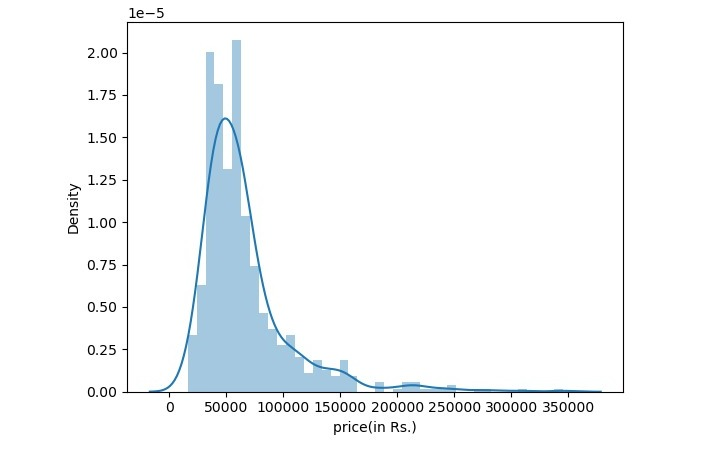
\includegraphics[width=6in]{1.png}
\caption{Analysis of price ranges for different Laptops}
\label{fig:dunnhalftone}
\end{figure} 
\begin{lstlisting}[language=Python]
import seaborn as sns
import pandas as pd
import  matplotlib.pyplot as plt
k=pd.read_csv("file2.csv")
plt.scatter(k['name'],k['ram'])
\end{lstlisting}
\vspace{5\baselineskip}
\begin{figure}[h]
\centering
 \footnotesize
 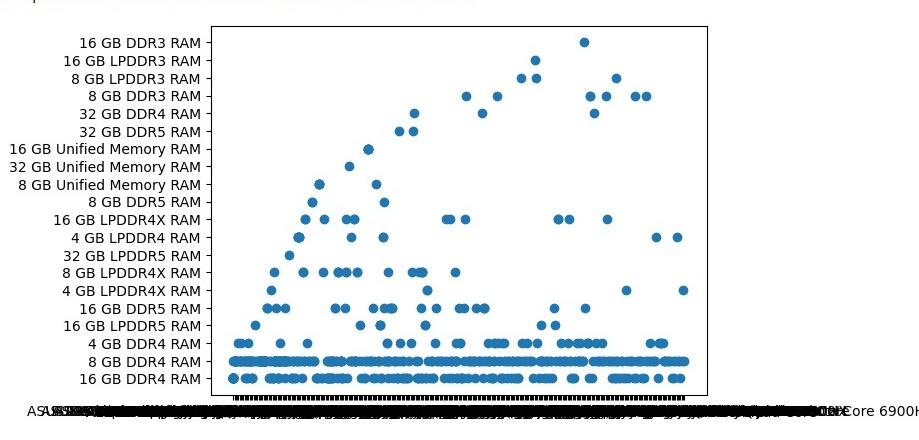
\includegraphics[width=6in]{2.png}
\caption{RAM Distribution}
\label{fig:dunnhalftone}
\end{figure} 
\begin{lstlisting}[language=Python]
import numpy as np
import pandas as pd
import  matplotlib.pyplot as plt
import seaborn as sns
p=sns.barplot(k['processor'],k['price(in Rs.)'])
\end{lstlisting}
 \begin{figure}[h]
\centering
 \footnotesize
 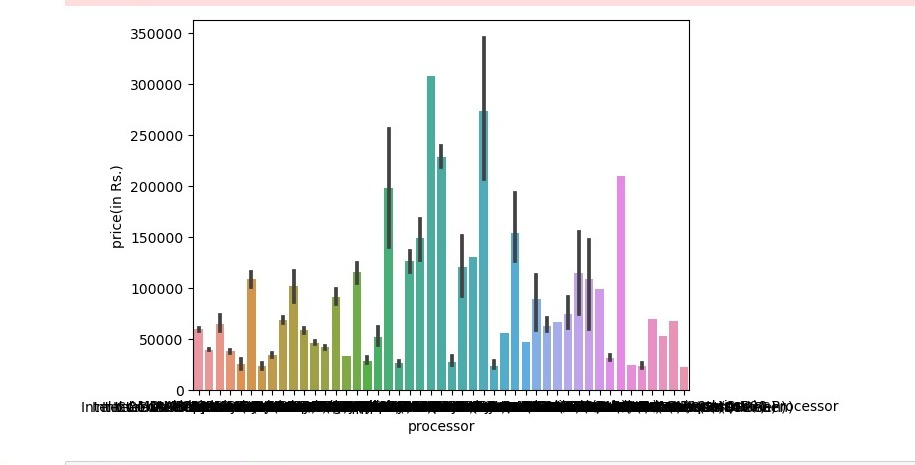
\includegraphics[width=6in]{3.png}
\caption{visual representation of the relationship between different processors and their prices.}
\label{fig:dunnhalftone}
\end{figure}
\begin{lstlisting}[language=Python]
import pandas as pd
import seaborn as sns
import  matplotlib.pyplot as plt
g=sns.JointGrid(x="rating",y="display(in inch)",data=d)
g=g.plot(sns.regplot,sns.distplot)
\end{lstlisting}
 \begin{figure}[h]
\centering
 \footnotesize
 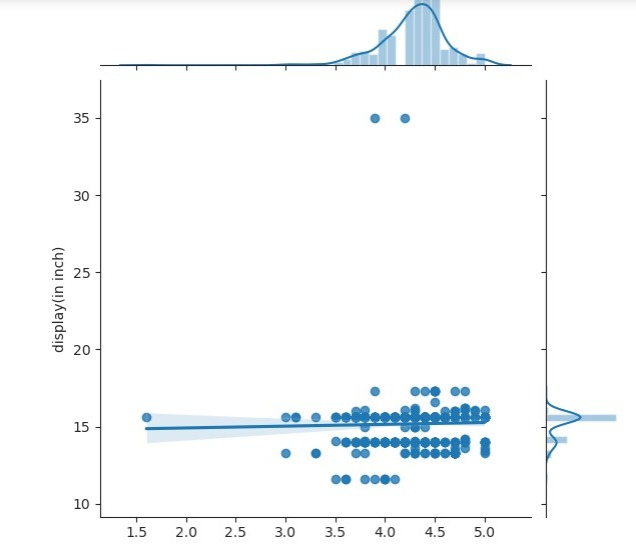
\includegraphics[width=4in]{4.png}
\caption{Distribution of ratings and display sizes}
\label{fig:dunnhalftone}
\end{figure} 


\begin{lstlisting}[language=Python]
import seaborn as sns
import pandas as pd
import  matplotlib.pyplot as plt
plt.figure(figsize=(12,6))
d.groupby('name').size().sort_values(ascending=False).head(5).plot(kind = 'bar',color = sns.color_palette('Paired'))
plt.xlabel('name of the laptop')
plt.ylabel('Number of Laptops')
plt.title('Top 5 most popular laptops brand')
plt.show()
\end{lstlisting}
\vspace{5\baselineskip}
\begin{figure}[h]
\centering
 \footnotesize
 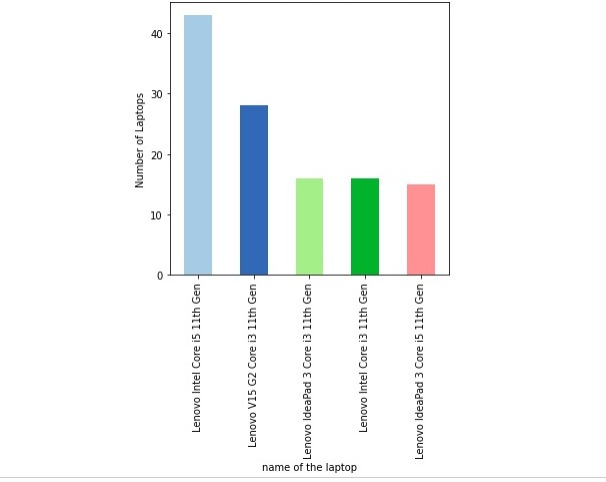
\includegraphics[width=4in]{5.png}
\caption{Top 5 most popular laptops brand}
\label{fig:dunnhalftone}
\end{figure} 
\begin{lstlisting}[language=Python]
import seaborn as sns
import pandas as pd
import  matplotlib.pyplot as plt
sns.boxplot(x="display(in inch)",y="rating",data=d)
plt.show()
\end{lstlisting}
\begin{figure}[h]
\centering
 \footnotesize
 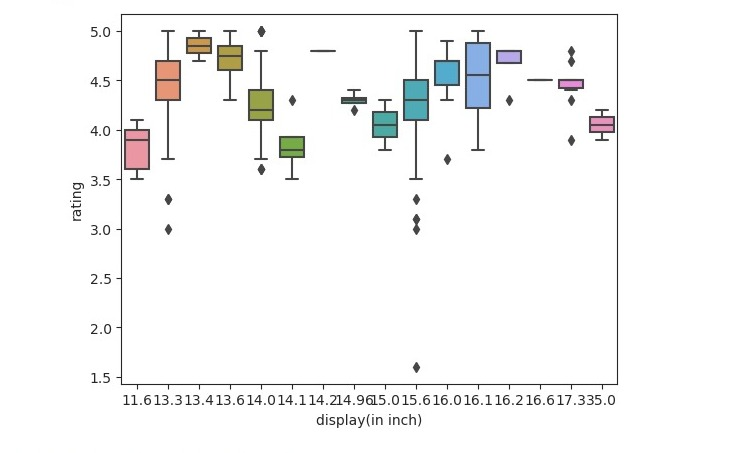
\includegraphics[width=4in]{7.png}
\caption{Example graph for box plot using seaborn }
\label{fig:dunnhalftone}
\end{figure} 
\begin{lstlisting}[language=Python]
import seaborn as sns
import pandas as pd
import  matplotlib.pyplot as plt
sns.violinplot(x=d["rating"])
plt.show()
\end{lstlisting}
\begin{figure}[h]
\centering
 \footnotesize
 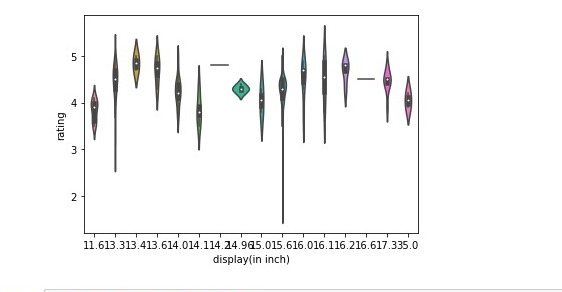
\includegraphics[width=4in]{8.png}
\caption{Distribution of ratings}
\label{fig:dunnhalftone}
\end{figure} 
\begin{lstlisting}[language=Python]
import seaborn as sns
import pandas as pd
import  matplotlib.pyplot as plt
plt.figure(figsize=(12,6))
d.groupby('ram').size().sort_values(ascending=False).plot(kind = 'bar',color = sns.color_palette('Blues'))
plt.xlabel('Ram Size in GB')
plt.ylabel('Number of Laptops')
plt.show()
\end{lstlisting}
\begin{figure}[h]
\centering
 \footnotesize
 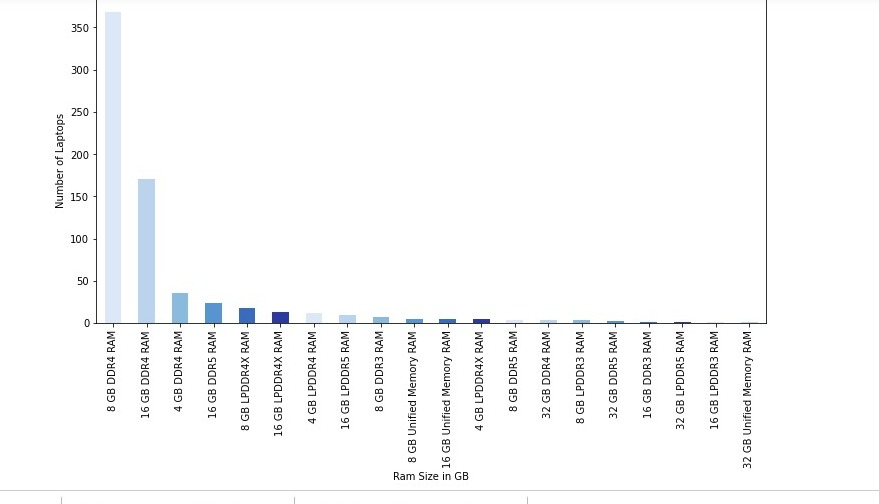
\includegraphics[width=4in]{9.png}
\caption{ graph shows the number of laptops for each RAM category}
\label{fig:dunnhalftone}
\end{figure} 

\begin{lstlisting}[language=Python]
import seaborn as sns
import pandas as pd
import  matplotlib.pyplot as plt
sns.set_style("ticks")
sns.pairplot(d)
plt.show()
\end{lstlisting}
\begin{figure}[h]
\centering
 \footnotesize
 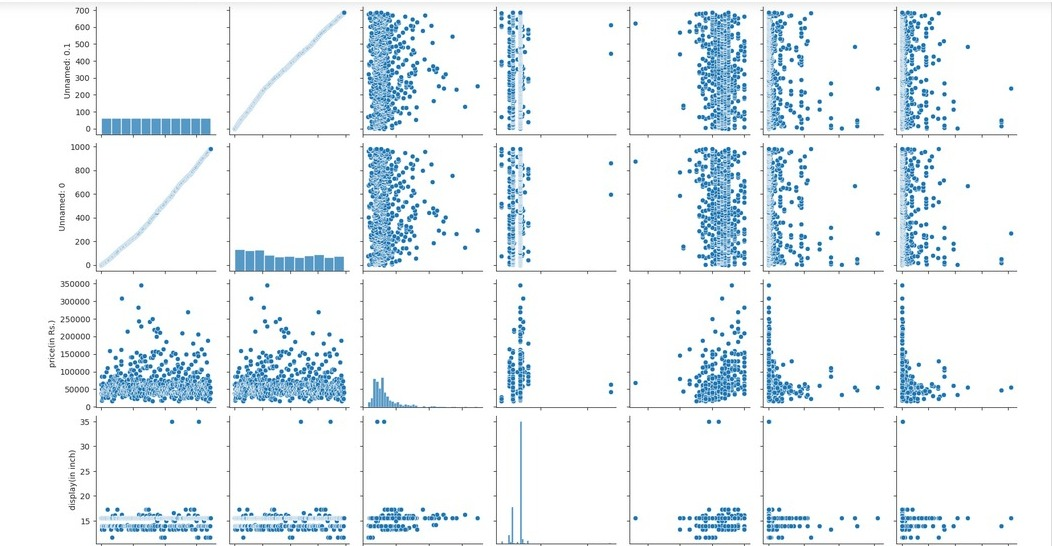
\includegraphics[width=4in]{11.png}
\caption{Relationships between variables}
\label{fig:dunnhalftone}
\end{figure} 
\begin{lstlisting}[language=Python]
import seaborn as sns
import pandas as pd
import  matplotlib.pyplot as plt
sns.distplot(d["price(in Rs.)"],kde=False)
plt.show()
\end{lstlisting}
\begin{figure}[h]
\centering
 \footnotesize
 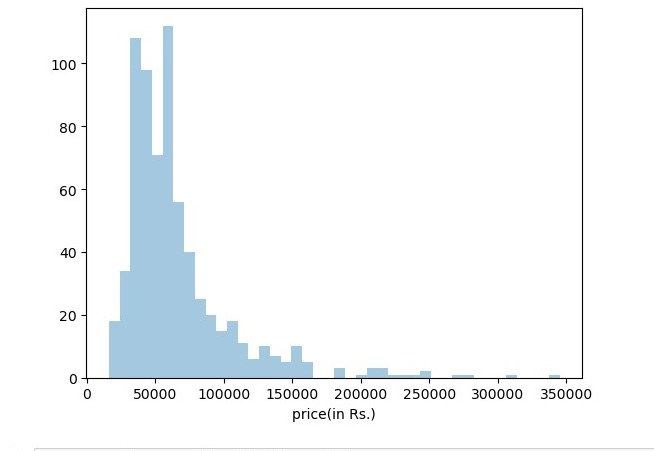
\includegraphics[width=4in]{12.png}
\caption{example graph of distplot}
\label{fig:dunnhalftone}
\end{figure} 

\section{Visualization} 
\begin{lstlisting}[language=Python]
plt.figure(figsize=(9,8))
sns.heatmap(d.corr(),square=True,annot=True,cmap="mako",center=0)
\end{lstlisting}
output:
\begin{figure}[h]
\centering
\footnotesize
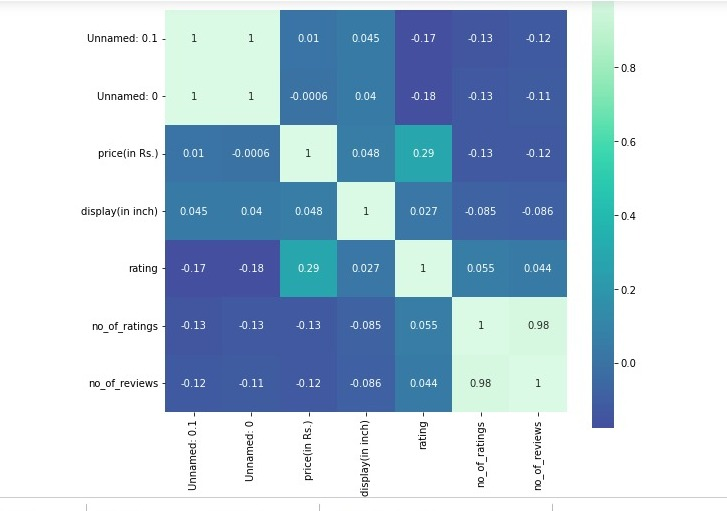
\includegraphics[width=8in]{13.jpeg}
\caption{Example for Heatmap}
\label{fig:unevenlight}
\end{figure}

 \begin{lstlisting}[language=Python]
 sns.regplot(x="rating",y="display(in inch)",data=d)
 plt.show()
 \end{lstlisting}
 \vspace{4\baselineskip}
 output:
\begin{figure}[h]
\centering
\footnotesize
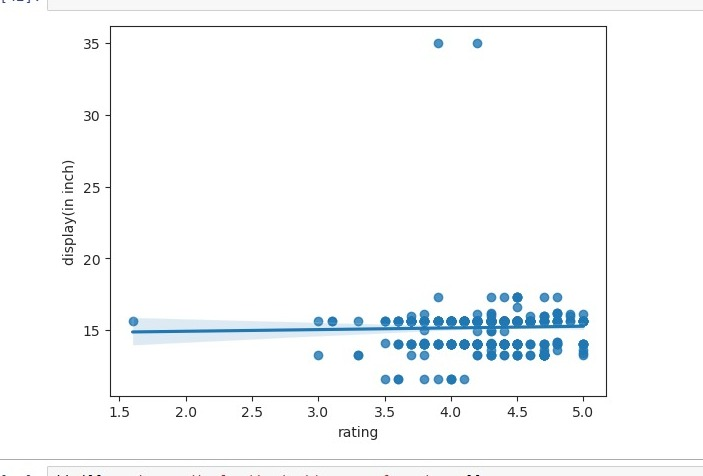
\includegraphics[width=4in]{15.png}
\caption{example graph for regplot}
\label{fig:unevenlight}
\end{figure}

\begin{lstlisting}[language=Python]
sns.distplot(d["rating"],hist=False)
plt.show()
 \end{lstlisting}
 output: 
\begin{figure}[h]
\centering
\footnotesize
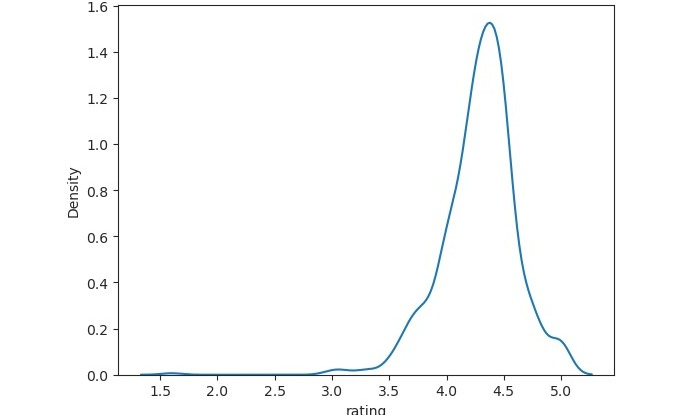
\includegraphics[width=5in]{16.png}
\caption{example graph for distplot}
\label{fig:unevenlight}
\end{figure}
 \vspace{4\baselineskip}

\begin{lstlisting}[language=Python]
sns.swarmplot(x="display(in inch)",y="rating",data=d)
plt.show()
 \end{lstlisting}
 output:
\begin{figure}[h]
\centering
\footnotesize
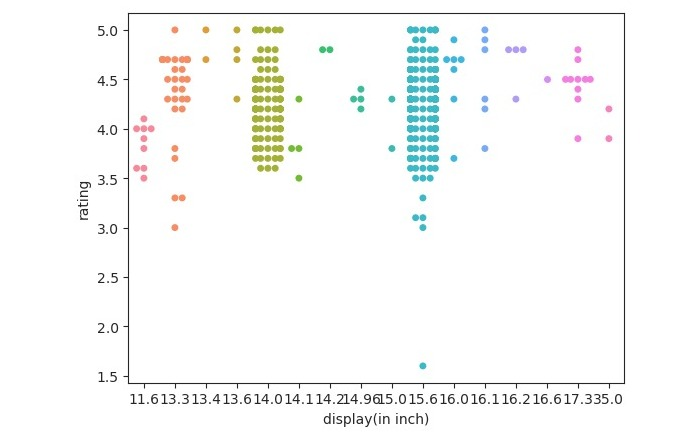
\includegraphics[width=6in]{17.jpeg}
\caption{  Example  of swarmplot}
\label{fig:unevenlight}
\end{figure}
This section contain minimum of 12 pages

\chapter{Code}
\section{Explain Your Code With Outputs}
\begin{figure}[h]
\centering
\footnotesize
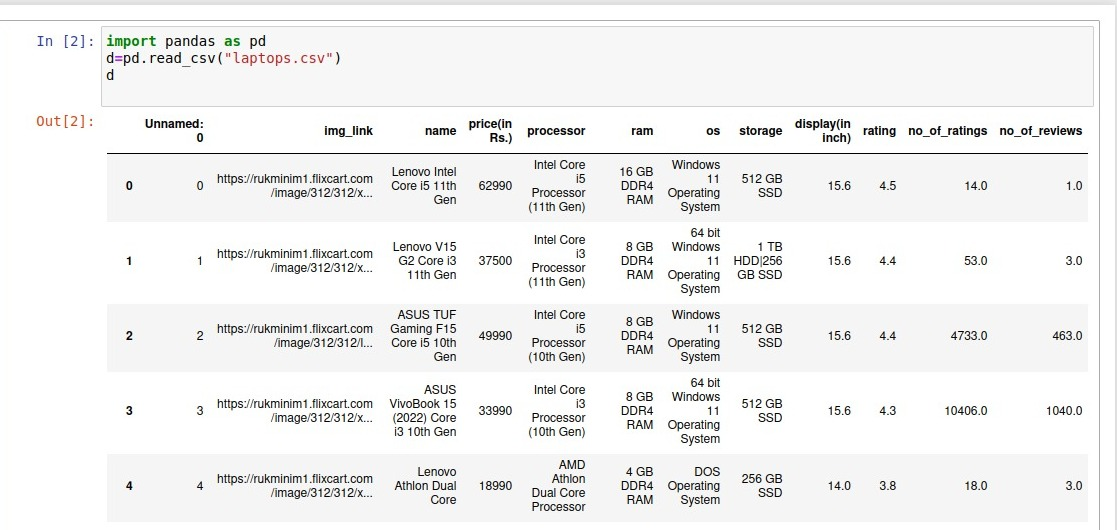
\includegraphics[width=7in]{20.jpeg}
\caption{csv file reading}
\label{fig:unevenlight}
\end{figure}

\vspace{4\baselineskip}
\begin{figure}[h]
\centering
\footnotesize
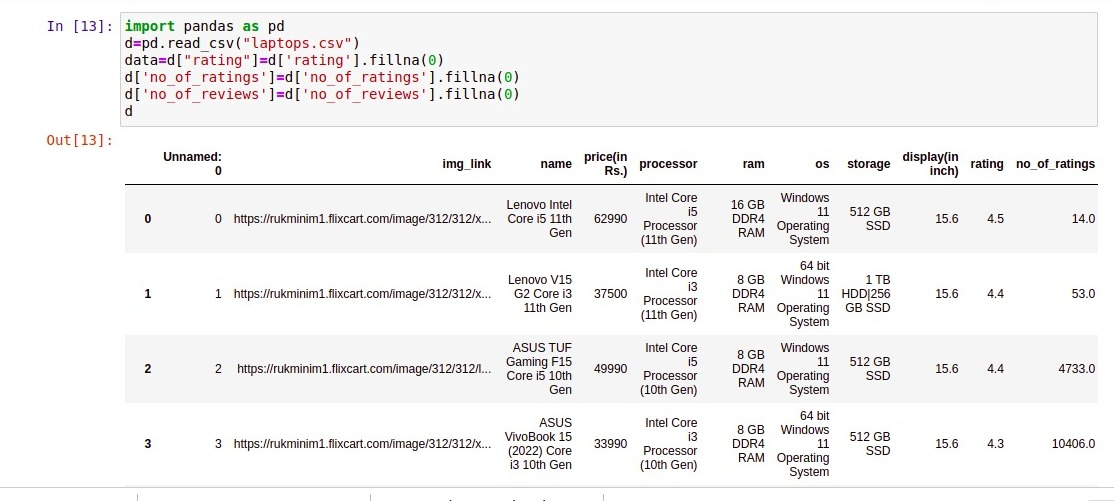
\includegraphics[width=6in]{21.jpeg}
\caption{filling the null values with 0}
\label{fig:unevenlight}
\end{figure}
\vspace{10\baselineskip}
\begin{figure}[h]
\centering
\footnotesize
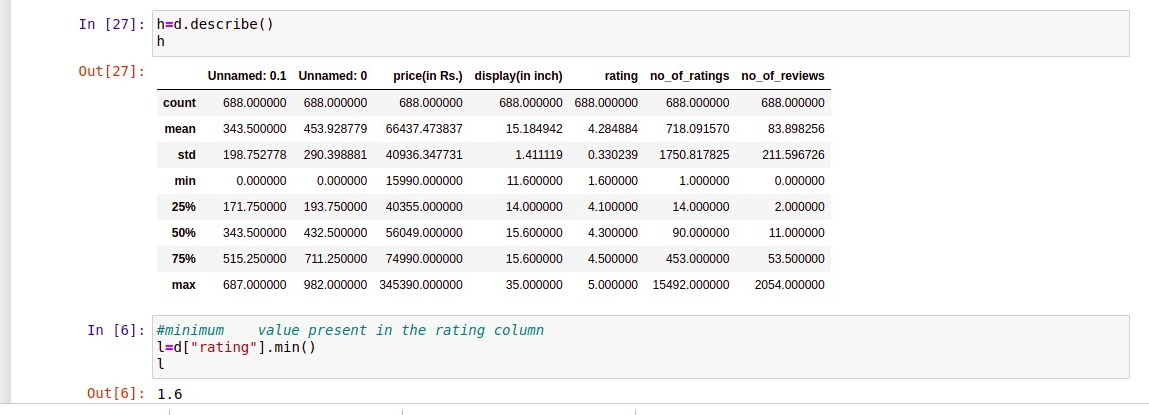
\includegraphics[width=9in]{22.jpeg}
\caption{stastical data}
\label{fig:unevenlight}
\end{figure}
\vspace{7\baselineskip}

\begin{figure}[h]
\centering
\footnotesize
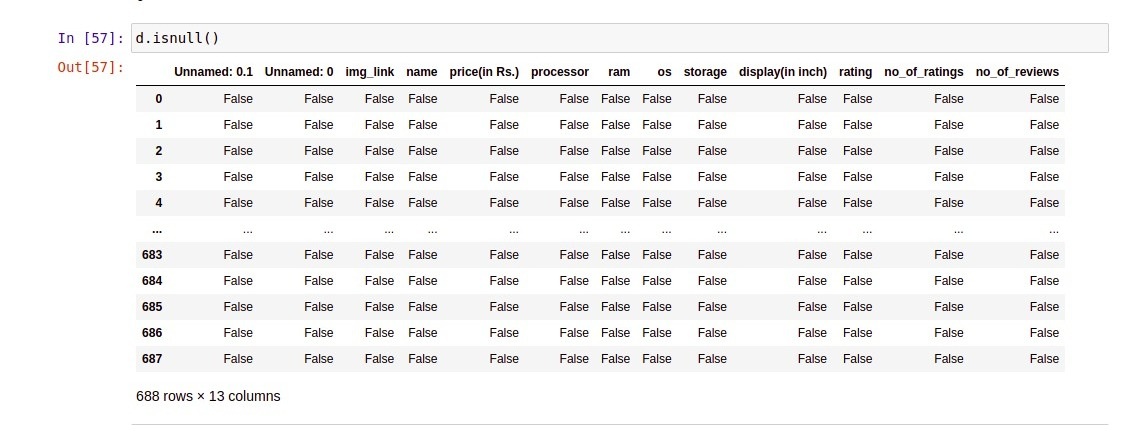
\includegraphics[width=7in]{23.jpeg}
\caption{finding Null values}
\label{fig:unevenlight}
\end{figure}
\vspace{7\baselineskip}

\begin{figure}[h]
\centering
\footnotesize
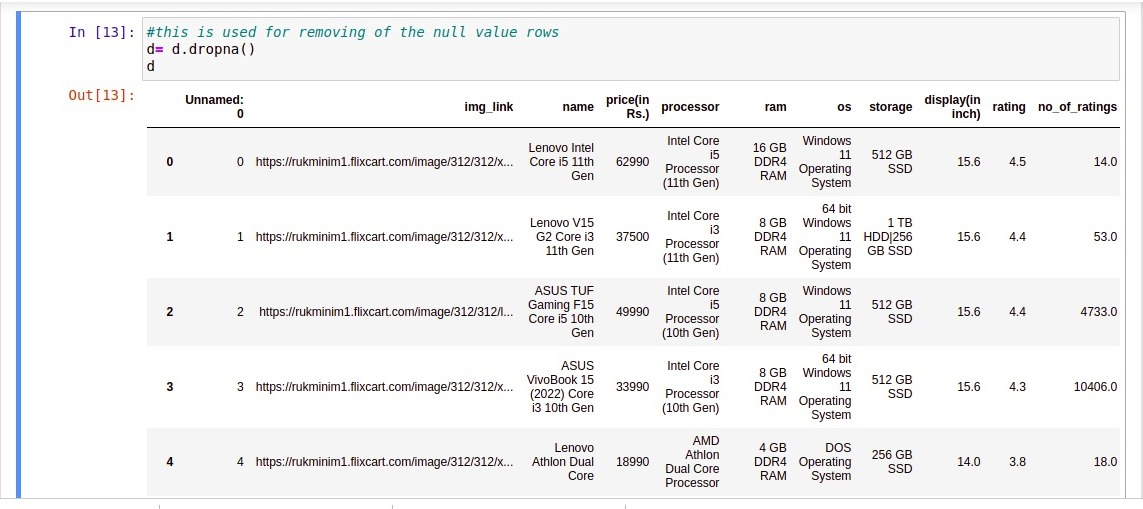
\includegraphics[width=7in]{28.jpeg}
\caption{Removing the null values containg rows}
\label{fig:unevenlight}
\end{figure}
\vspace{9\baselineskip}



\begin{figure}[h]
\centering
\footnotesize
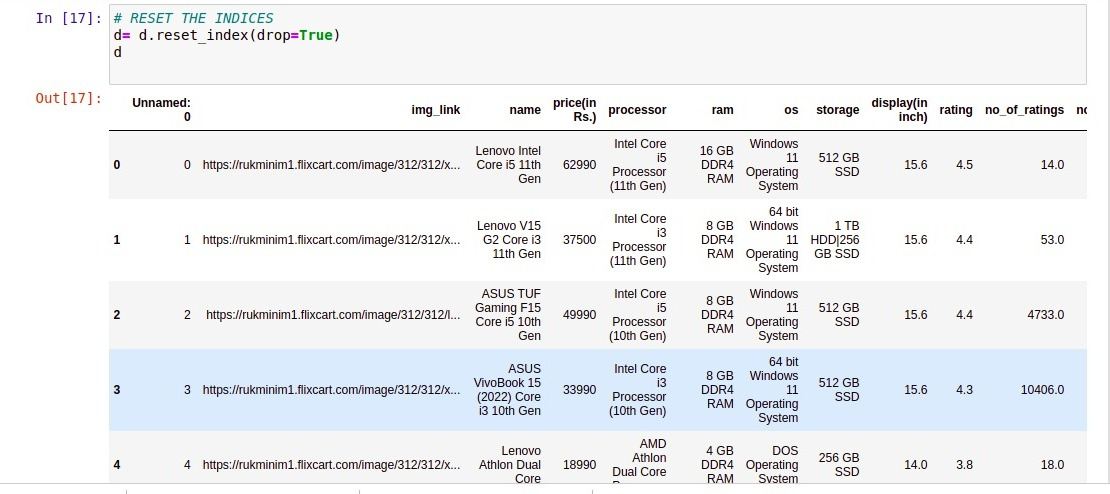
\includegraphics[width=7in]{29.jpeg}
\caption{Reset the indices}
\label{fig:unevenlight}
\end{figure}
\vspace{5\baselineskip}
\begin{figure}[h]
\centering
\footnotesize
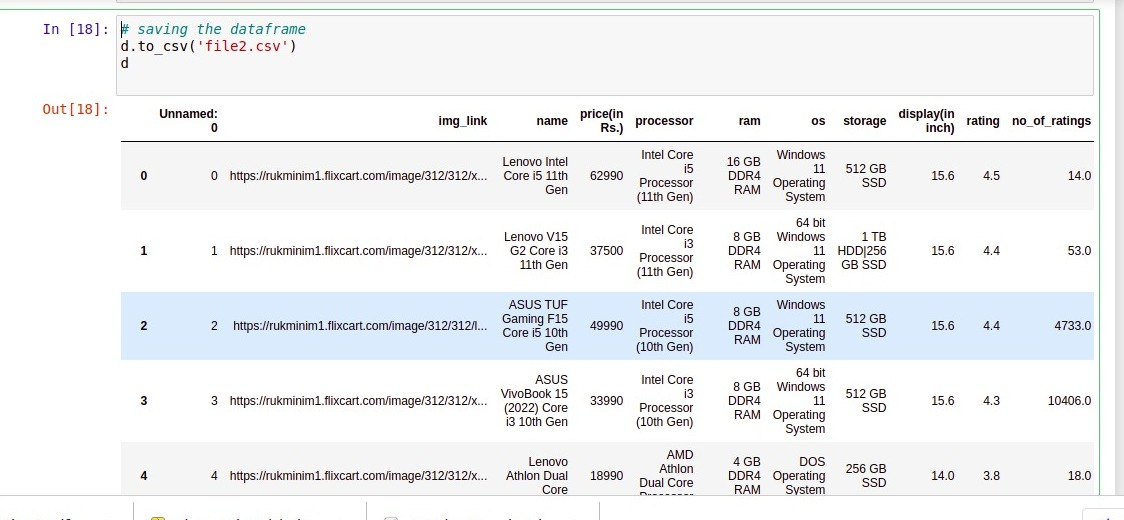
\includegraphics[width=6in]{30.jpeg}
\caption{After data processing saving dataframe into csv file }
\label{fig:unevenlight}
\end{figure}
\vspace{7\baselineskip}

\begin{figure}[h]
\centering
\footnotesize
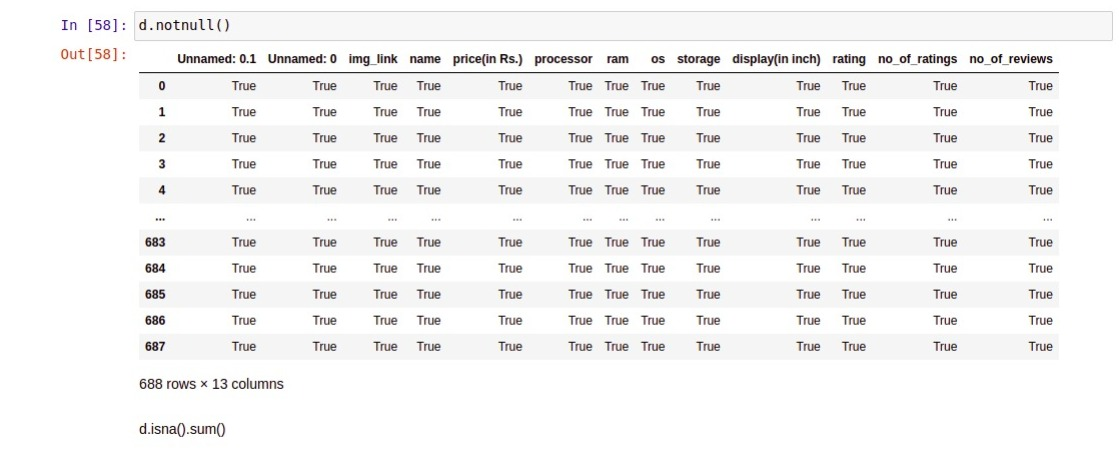
\includegraphics[width=7in]{24.jpeg}
\caption{checking the null values}
\label{fig:unevenlight}
\end{figure}

\begin{lstlisting}[language=Python]
import pandas as pd
import numpy as np
k=pd.read_csv("file2.csv")
k=pd.DataFrame(k)
k.sort_values(['price(in Rs.)'], inplace=True)
categorical_features =k.columns[(k.dtypes == 'object') == True].to_list()
print(categorical_features)
for feature in categorical_features:
    uniq = k[feature].unique()
    new_feature = []
    for el in k[feature]:
        new_feature.append(len(uniq) - np.where(uniq==el)[0][0])
    k[feature] = new_feature   
k
from sklearn.model_selection import train_test_split
from sklearn.ensemble import RandomForestClassifier
from sklearn.metrics import accuracy_score
from sklearn import metrics
from sklearn.metrics import mean_absolute_error, mean_squared_error, r2_score
import  matplotlib.pyplot as plt
import seaborn as sb
x=k.drop(['price(in Rs.)'], axis=1)
y=k["price(in Rs.)"].values
x_train, x_test, y_train, y_test = train_test_split(x, y, test_size=0.3, random_state=42)
rf_classifier = RandomForestClassifier(n_estimators=100)
rf_classifier.fit(x_train, y_train)
y_pred = rf_classifier.predict(x_test)
# Calculate accuracy
accuracy = accuracy_score(y_test, y_pred)
print("accuracy: ",accuracy)
MAE = mean_absolute_error(y_test, y_pred)
MSE = mean_squared_error(y_test, y_pred)
R2 = r2_score(y_test, y_pred)
print("Mean Absolute Error:", MAE)
print("Mean Squared Error:", MSE)
print("R-squared:", R2)
output:
\end{lstlisting}
\begin{figure}[h]
\centering
\footnotesize
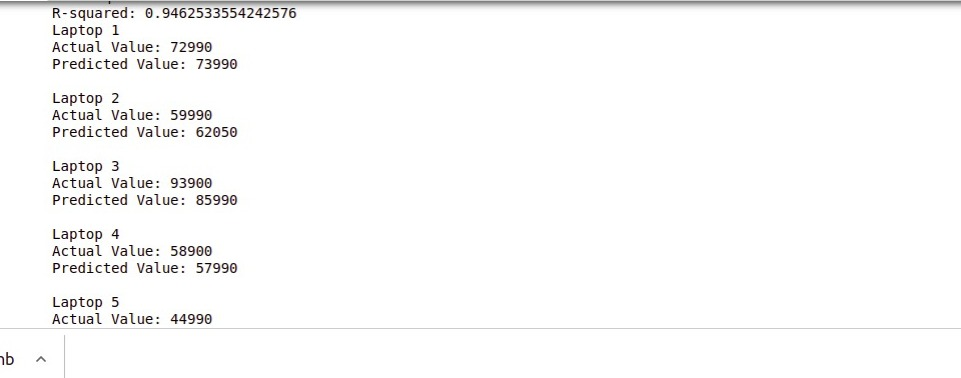
\includegraphics[width=6in]{56.jpeg}
\label{fig:unevenlight}
\end{figure}
\begin{lstlisting}[language=Python]
plt.scatter(y_test, y_pred)
plt.xlabel('Actual Values')
plt.ylabel('Predicted Values')
plt.title('Actual vs Predicted Values')
plt.show()
 \end{lstlisting} 
 output:    
\begin{figure}[h]
\centering
\footnotesize
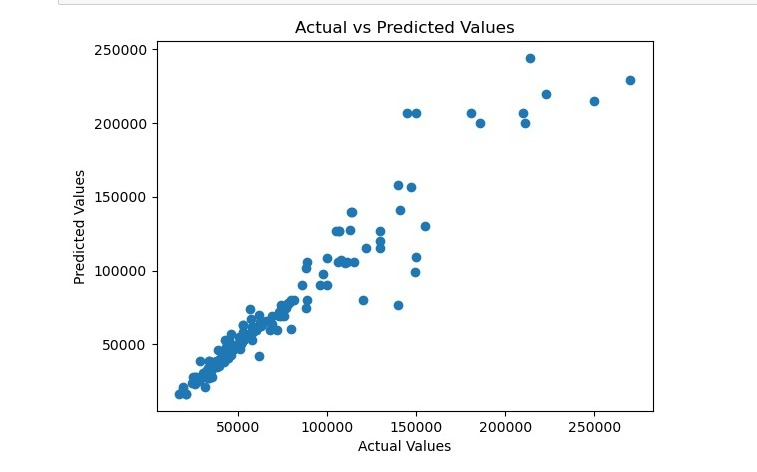
\includegraphics[width=5in]{35.jpeg}
\label{fig:unevenlight}
\end{figure}  

\begin{lstlisting}[language=Python]
\
plt.plot(range(len(y_test)), y_test, color='blue', label='Actual')
plt.plot(range(len(y_pred)), y_pred, color='red', label='Predicted')
plt.xlabel('Data Point Index')
plt.ylabel('Price')
plt.legend()
plt.show()
\end{lstlisting}
 \begin{figure}[h]
\centering
\footnotesize
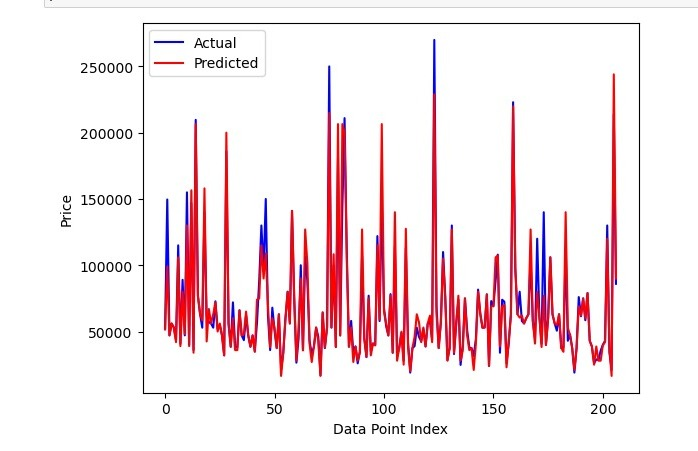
\includegraphics[width=3in]{31.png}
\caption{Actual vs Predicted values}
\label{fig:unevenlight}
\end{figure}
\vspace{2\baselineskip}
\begin{lstlisting}[language=Python]
plt.scatter(range(len(y_test)), y_test, color='blue', label='Actual')
plt.scatter(range(len(y_pred)), y_pred, color='red', label='Predicted')
plt.plot(range(len(y_pred)), y_pred, color='green', linewidth=2, label='Best Fit Line')
plt.xlabel('Data Point Index')
plt.ylabel('Price')
plt.legend()
plt.show()
\end{lstlisting}
output: 
\begin{figure}[h]
\centering
\footnotesize
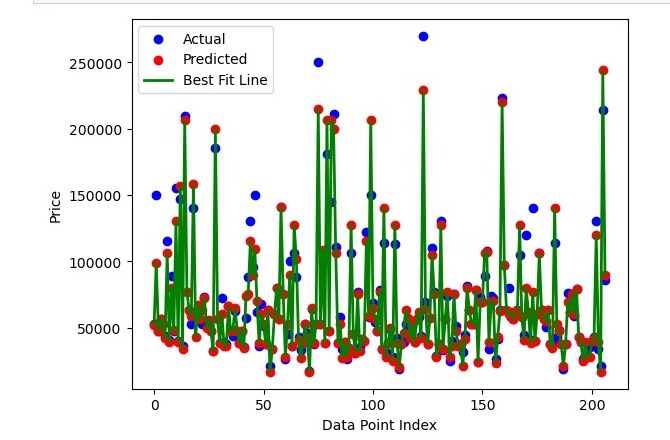
\includegraphics[width=6in]{33.jpeg}
\caption{Best Fit Line For Actual vs Predicted Values}
\label{fig:unevenlight}
\end{figure} 
 \begin{lstlisting}[language=Python]
plt.scatter(range(len(y_test)), y_test, color='blue', label='Actual')
plt.scatter(range(len(y_pred)), y_pred, color='red', label='Predicted')
plt.xlabel('Data Point Index')
plt.ylabel('Price')
plt.legend()
plt.show()
 \end{lstlisting} 
 output: 
 \begin{figure}[h]
\centering
\footnotesize
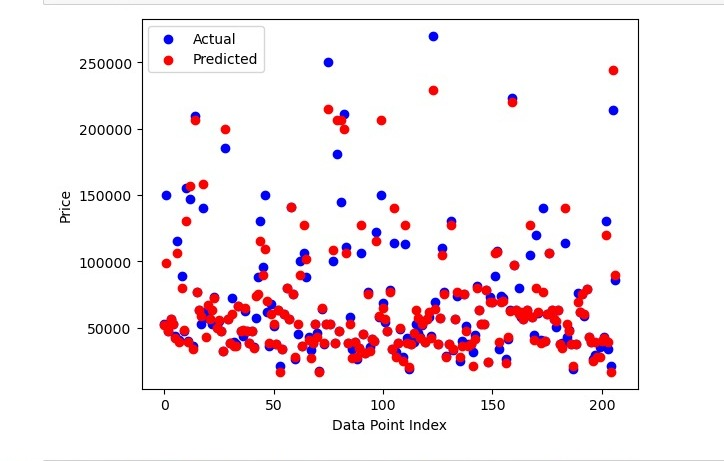
\includegraphics[width=4in]{34.jpeg}
\caption{scatter plot for  actual price vs predicted price }
\label{fig:unevenlight}
\end{figure}
\begin{lstlisting}[language=Python]
import pandas as pd
from sklearn.ensemble import RandomForestClassifier
k = pd.read_csv('file2.csv') 

categorical_features = k.columns[(k.dtypes == 'object') == True].to_list()
print(categorical_features)
for feature in categorical_features:
    uniq = k[feature].unique()

    new_feature = []
    for el in k[feature]:
        new_feature.append(len(uniq) - np.where(uniq == el)[0][0])

    k[feature] = new_feature

features = ['storage', 'ram', 'os'] 
target = 'name' 
X = k[features]
y = k[target]

rf_classifier = RandomForestClassifier(n_estimators=100)
rf_classifier.fit(X, y)

new_features = ["11", "15", "20"]
new_laptop = pd.DataFrame([new_features], columns=features)
prediction = rf_classifier.predict(new_laptop)
selected_laptop = k[k[target] == prediction[0]]

print("Selected Laptop:")
print(selected_laptop)
\end{lstlisting}
\begin{figure}[h]
\centering
\footnotesize
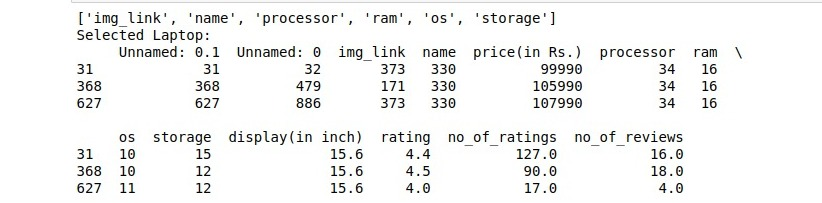
\includegraphics[width=5in]{54.jpeg}
\label{fig:unevenlight}
\end{figure}
\begin{lstlisting}[language=Python]
import pandas as pd
from sklearn.model_selection import train_test_split
from sklearn.ensemble import RandomForestRegressor
from sklearn.metrics import accuracy_score
from sklearn.metrics import mean_squared_error, r2_score
X=k.drop(['price(in Rs.)'], axis=1)
y=k["price(in Rs.)"].values
X_train, X_test, y_train, y_test = train_test_split(X, y, test_size=0.2, random_state=42)
rf = RandomForestRegressor()
rf.fit(X_train, y_train)
y_pred = rf.predict(X_test)
mse = mean_squared_error(y_test, y_pred)
r2 = r2_score(y_test, y_pred)
print('Mean Squared Error:', mse)
print('R-squared:', r2)
print("Actual values:")
print(y_test)
print("Predicted values:")
print(y_pred)
output:
R-squared value:0.9740704887906095
\end{lstlisting}







\chapter{Conclusion and Future Work}

In conclusion, a laptop selection and price prediction project aims to assist users in making informed decisions when choosing a laptop by estimating its price based on its specifications. The project involves several key steps, including data collection, preprocessing, feature selection, model training, evaluation, and prediction.
By analyzing features such as brand, model, processor, RAM, storage, display size, and others, machine learning models can be trained to predict the price of a laptop. Regression techniques like linear regression, decision trees, random forests, or gradient boosting are commonly used for price prediction. Classification techniques can also be valuable for categorizing laptops based on price ranges, feature importance, brand, laptop type, or sentiment analysis.
Through the laptop selection and price prediction process, users can benefit from a better understanding of the factors influencing laptop prices and the ability to compare different laptops based on their preferences and budget constraints. The project provides a valuable tool to assist users in selecting the most suitable laptop for their specific needs and helps them make informed purchasing decisions.
It's important to note that while machine learning models can provide price estimates, actual laptop prices may still vary due to various factors such as market trends, discounts, or economic variables. The accuracy of the price prediction models depends on the quality and representativeness of the dataset, the choice of features, and the chosen machine learning techniques.
Overall, a laptop selection and price prediction project helps users navigate the wide range of laptops available in the market by providing estimates of their prices based on specifications. This empowers users to make well-informed decisions and find laptops that best meet their requirements and budget.

\end{document}
